\documentclass[10pt]{article}


\usepackage[margin=1in]{geometry}
\usepackage{amsmath,amssymb}
\usepackage{wrapfig}
\usepackage{multicol}
\usepackage{graphicx}
\usepackage{makecell}
\usepackage{moresize}
\usepackage{lmodern}
\usepackage{tikz}

\graphicspath{{figs/}}
\newcommand{\sect}[1]{\noindent\textbf{#1}\\}
\newcommand{\hl}{\noindent\makebox[\linewidth]{\rule{\textwidth}{0.2pt}}}
\newcommand\tab[1][1cm]{\hspace*{#1}}
\newcommand{\nin}{\noindent}

\DeclareMathOperator{\sinc}{sinc}

\setlength{\columnsep}{1.5cm}
\setlength{\columnseprule}{0.2pt}

\begin{document}
	
	\begin{ssmall}
	\begin{multicols*}{2}
	\nin{\normalsize \textbf{Test \#1 Equation Sheet:}}
	
	\sect{Even/Odd Components:}
	
	\nin $x_{odd} = \cfrac{x(t)-x(-t)}{2}$
	
	\nin $x_{even} = \cfrac{x(t)+x(-t)}{2}$\\
	
	\sect{Energy and Power:}
	\nin $E_{a,b} = \int_a^b |x(t)|^2 dt$
	
	\nin $P_{a,b} = \cfrac{1}{b-a} \int_a^b |x(t)|^2 dt = \cfrac{E_{a,b}}{b-a}$\\
	
	\sect{Rotating Phasors:}
	\nin $x(t) = A \cos(\omega_0 t + \theta)$
	
	\nin $\tilde{x}(t) = A e^{\omega_0 t + \theta}$
	
	\nin $x(t) = \cfrac{\tilde{x}(t) + \tilde{x}^*(t)}{2}$\\
	
	\sect{Double Sided Spectrum:}
	\nin $x(t) = \cfrac{A}{2}e^{j\theta}e^{j(\omega_0 t)} + \cfrac{A}{2} e^{-j\theta}e^{j(-\omega_0 t)}$
	
	\nin \begin{tikzpicture}[scale=0.2, every node/.style={scale=0.25}]
	\draw (0, 5) -- (15, 5);
	\draw (7.5, 0) -- (7.5, 10);
	\draw (7, 9.5) -- (8, 9.5) node[right]{{\HUGE$\cfrac{A}{2}$}};
	\draw (3.75, 5.5) -- (3.75, 4.5) node[below]{{\HUGE $-f_0$ }}; 
	\draw (11.25, 5.5) -- (11.25, 4.5) node[below]{{\HUGE $f_0$ }};
	\draw (3.75, 5) -- (3.75, 9.5) node[circle, fill, inner sep=3pt]{};
	\draw (11.25, 5) -- (11.25, 9.5) node[circle, fill, inner sep=3pt]{};
	\end{tikzpicture} 
	\tab[0.25cm] \begin{tikzpicture}[scale=0.2, every node/.style={scale=0.25}]
	\draw (0, 5) -- (15, 5);
	\draw (7.5, 0) -- (7.5, 10);
	\draw (7, 9.5) -- (8, 9.5) node[right]{{\HUGE$\theta$}};
	\draw (7, 0.5) -- (8, 0.5) node[right]{{\HUGE$-\theta$}};
	\draw (3.75, 5.5) -- (3.75, 4.5) node[below]{{\HUGE $-f_0$ }}; 
	\draw (11.25, 5.5) node[above]{{\HUGE $f_0$ }} -- (11.25, 4.5);
	\draw (3.75, 5) -- (3.75, 9.5) node[circle, fill, inner sep=3pt]{};
	\draw (11.25, 5) -- (11.25, 0.5) node[circle, fill, inner sep=3pt]{};
	\end{tikzpicture}
	
	\nin $\omega_0 = 2\pi f_0$, \tab[0.1cm] $f_0 = \cfrac{1}{T_0}$\\
	
	\sect{$\delta(t) Properties$}
	$\delta(at) = \cfrac{1}{|a|} \delta(t)$
	
	\nin $\delta(t) = \delta(-t)$
	
	\nin $\int_a^b x(t)\delta(t-t_0) = \left\{
	\begin{aligned}
		x(t_0) &\text{ \tab[0.1cm] if } a \leq t_0 \leq b \\
		0 &\text{ \tab[0.1cm] else}
	\end{aligned}\right.$
	
	\nin $x(t) \delta(t-t_0) = x(t_0) \delta(t-t_0)$
	
	\nin $\delta(t) = \cfrac{d}{dt} u(t)$\\
	
	\sect{Properties of Systems:}
	Linear: Scaling and Additive must hold, i.e.\\
	$\begin{aligned}
	y_1(t) &= H\left\{x_1(t)\right\}\\
	y_2(t) &= H\left\{x_2(t)\right\}
	\end{aligned} \Rightarrow H\left\{\alpha x_1 + \beta x_2\right\} = \alpha y_1 + \beta y_2$\\
	
	\nin Time Invariant: Shift by the same amount, i.e.\\
	$y(t) = H\left\{x(t)\right\} \Rightarrow H\left\{x(t-\tau)\right\} = y(t-\tau)$\\
	
	\nin Causal: Output begins at the same same time or after, i.e.\\
	$x_1 = x_2 \text{ for } t \leq t_0 \Rightarrow H\left\{x_1\right\} = H\left\{x_2\right\} \text{ for } t \leq t_0$\\
	
	\nin Stable: Bounded Input $\Rightarrow$ Bounded Output\\
	
	\sect{Convolution:}
	$y\left[n\right] = x\left[n\right] \ast h[n] = \sum\limits_{k=-\infty}^{\infty} x[k]h[n-k]$, \tab[0.1cm] $h[n] = H\{\delta[n]\}$
	
	\nin $y(t) = x(t) \ast h(t) = \int_{-\infty}^{\infty} x(t)h(t-\lambda)d\lambda$,\tab[0.1cm] $h(t) = H\{\delta(t)\}$
	
	\nin Graphical Representation:
	
	\nin 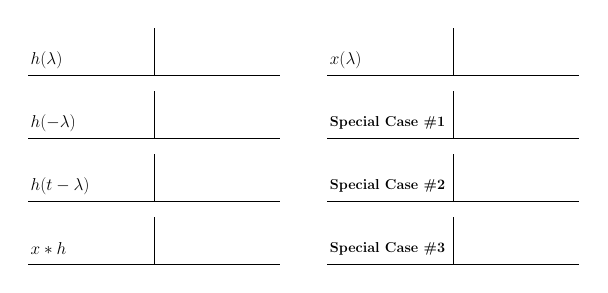
\begin{tikzpicture}[scale=0.2, every node/.style={scale=0.25}]
	\def\len{16}
	\def\sep{3}
	\def\height{3}
	\def\vertsep{1}
	
	\draw (0, 0) -- (\len,0);
	\draw (0, \height + \vertsep) -- (\len, \height + \vertsep);
	\draw (0, 2*\height + 2*\vertsep) -- (\len, 2*\height + 2*\vertsep);
	\draw (0, 3*\height + 3*\vertsep) -- (\len, 3*\height +3*\vertsep);
	
	\draw (\len + \sep, 0) -- (2*\len + \sep, 0);
	\draw (\len + \sep, \height + \vertsep) -- (2*\len + \sep, \height + \vertsep);
	\draw (\len + \sep, 2*\height + 2*\vertsep) -- (2*\len + \sep, 2*\height + 2*\vertsep);
	\draw (\len + \sep, 3*\height + 3*\vertsep) -- (2*\len + \sep, 3*\height + 3*\vertsep);
	
	\draw (0.5*\len, 0) -- (0.5*\len, \height);
	\draw (0.5*\len, \height+\vertsep) -- (0.5*\len, 2*\height+\vertsep);
	\draw (0.5*\len, 2*\height+2*\vertsep) -- (0.5*\len, 3*\height+2*\vertsep);
	\draw (0.5*\len, 3*\height+3*\vertsep) -- (0.5*\len, 4*\height+3*\vertsep);
	
	\draw (1.5*\len + \sep, 0) -- (1.5*\len + \sep, \height);
	\draw (1.5*\len + \sep, \height+\vertsep) -- (1.5*\len + \sep, 2*\height+\vertsep);
	\draw (1.5*\len + \sep, 2*\height+2*\vertsep) -- (1.5*\len + \sep, 3*\height+2*\vertsep);
	\draw (1.5*\len + \sep, 3*\height+3*\vertsep) -- (1.5*\len + \sep, 4*\height+3*\vertsep);
	
	\draw (0, 4*\height + 3*\vertsep - 2) node[right]{\HUGE$h(\lambda)$};
	\draw (0, 3*\height + 2*\vertsep - 2) node[right]{\HUGE$h(-\lambda)$};
	\draw (0, 2*\height + \vertsep - 2) node[right]{\HUGE$h(t-\lambda)$};
	\draw (0, \height - 2) node[right]{\HUGE$x \ast h$};
	
	\draw (\len+\sep, 4*\height + 3*\vertsep - 2) node[right]{\HUGE$x(\lambda)$};
	\draw (\len+\sep, 3*\height + 2*\vertsep - 2) node[right]{\huge \textbf{Special Case \#1}};
	\draw (\len+\sep, 2*\height + \vertsep - 2) node[right]{\huge \textbf{Special Case \#2}};
	\draw (\len+\sep, \height - 2) node[right]{\huge \textbf{Special Case \#3}};
	\end{tikzpicture}\\
	
	\sect{Circuit Equations: }
	Capacitors: $\begin{aligned}
	v_c &= \cfrac{1}{C} \textstyle\int i_c dt \\
	i_c &= C \cfrac{d v_c}{dt}
	\end{aligned}$\\\\
	
	\nin Inductors: $\begin{aligned}
	v_L &= L \cfrac{di_L}{dt}\\
	i_L &= \cfrac{1}{L} \textstyle \int v_L dt
	\end{aligned}$
	
	\nin{\normalsize \textbf{Test \#2 Equation Sheet:}}
	
	\sect{Trigonometric Fourier Series:}
	\nin $x(t) = a_0 + \sum\limits_{n=1}^{\infty} a_n cos(n \omega_0 t) + \sum\limits_{n=1}^{\infty} b_n sin(n \omega_0 t)$
	
	\nin $a_0 = \cfrac{1}{T_0}\displaystyle\int_{T_0}{x(t)dt}$ 
	
	\nin $a_n = \cfrac{2}{T_0}\displaystyle\int_{T_0}{x(t)cos(n \omega_0 t) dt}$
	
	\nin $b_n = \cfrac{2}{T_0}\displaystyle\int_{T_0}{x(t)sin(n \omega_0 t) dt}$\\
	
	\sect{Complex Exponential Fourier Series:}
	
	\nin $x(t) = \sum\limits_{n=-\infty}^{\infty} X_n e^{j n \omega_0 t}$
	
	\nin $X_n = \cfrac{1}{T_0} \displaystyle\int_{T_0} x(t) e^{-j n \omega_0 t} dt$
	
	\nin \begin{tabular}{|c|c|}
		\hline
		$x(t)$ & $X_n$ \\ \hline
		real & even mag., odd phase \\
		real and even & even mag. and purely real \\
		real and odd & even mag. and purely imaginary \\ \hline
	\end{tabular}\\

	\sect{Relationship between complex and trig Fourier Series:}
	\nin $a_0 = X_0$
	
	\nin $a_n = X_n + X_{-n}$
	
	\nin $b_n = j[X_n - X_{-n}]$
	
	\sect{Average power of a signal (Parseval's Theorem):}
	\nin $\cfrac{1}{T_0}\displaystyle\int_{t_0}^{t_0+T_0} | x(t) |^2 dt = \sum\limits_{n=-\infty}^{\infty} | X_n | ^2$\\
	
	\sect{The Fourier Transform:}
	\nin $X(f) = \displaystyle \int_{-\infty}^{\infty} x(t) e^{-j 2 \pi f t} dt \Longleftrightarrow x(t) = \displaystyle\int_{-\infty}^{\infty} X(f) e^{j 2 \pi f t} dt$\\
	
	\sect{Rayleigh's Energy Theorem:}
	\nin $E = \displaystyle\int_{-\infty}^{\infty} |x(t)|^2 dt = \int_{-\infty}^{\infty} | X(f) |^2 df$\\
	
	\sect{The Important Problem: {\tiny(Works for all sinusoids)}}
	\nin $y(t) = h(t) \ast A\cos(2\pi f_0 t + \theta) = A|H(f_0)|\cos(2\pi f_0t + \theta + \angle H(f_0))$\\
	
	\sect{Ideal Filters: {\tiny(impossible to create because they're not causal.)}}
	\nin \begin{tabular}{|c|c|c|}
		\hline
		Filter & H(f) & h(t) \\ \hline
		LPF & $\Pi \left(\frac{f}{2f_c}\right)$ & $(2 f_c) \sinc(2 f_c t)$ \\ \hline
		HPF & $1 - \Pi \left(\frac{f}{2f_c}\right)$ & $\delta(t) - (2f_c) \sinc{2f_ct}$ \\ \hline
		BPF & $\Pi\left(\frac{f-f_0}{B}\right) + \Pi\left(\frac{f+f_0}{B}\right)$ & $2B\sinc(Bt)\cos(2\pi f_0 t)$ \\ \hline
		BRF & $1-\Pi\left(\frac{f-f_0}{B}\right)  \Pi\left(\frac{f+f_0}{B}\right)$ & $\delta(t) - 2B\sinc(Bt)\cos(2\pi f_0 t)$ \\ \hline
	\end{tabular}\\

	\sect{Inductors and Capacitors:}
	\nin \begin{tabular}{|c|c|c|}
		\hline
		Variable & Inductor & Capacitor \\ \hline
		v(t) & $L \cfrac{di(t)}{dt}$ & $\cfrac{1}{C}\displaystyle\int i(t) dt$ \\ \hline
		i(t) & $\cfrac{1}{L}\displaystyle\int v(t) dt$ & $C \cfrac{d v(t)}{dt}$ \\ \hline
	\end{tabular}

	\end{multicols*}
	\end{ssmall}
\end{document}